\documentclass[1p]{elsarticle_modified}
%\bibliographystyle{elsarticle-num}

%\usepackage[colorlinks]{hyperref}
%\usepackage{abbrmath_seonhwa} %\Abb, \Ascr, \Acal ,\Abf, \Afrak
\usepackage{amsfonts}
\usepackage{amssymb}
\usepackage{amsmath}
\usepackage{amsthm}
\usepackage{scalefnt}
\usepackage{amsbsy}
\usepackage{kotex}
\usepackage{caption}
\usepackage{subfig}
\usepackage{color}
\usepackage{graphicx}
\usepackage{xcolor} %% white, black, red, green, blue, cyan, magenta, yellow
\usepackage{float}
\usepackage{setspace}
\usepackage{hyperref}

\usepackage{tikz}
\usetikzlibrary{arrows}

\usepackage{multirow}
\usepackage{array} % fixed length table
\usepackage{hhline}

%%%%%%%%%%%%%%%%%%%%%
\makeatletter
\renewcommand*\env@matrix[1][\arraystretch]{%
	\edef\arraystretch{#1}%
	\hskip -\arraycolsep
	\let\@ifnextchar\new@ifnextchar
	\array{*\c@MaxMatrixCols c}}
\makeatother %https://tex.stackexchange.com/questions/14071/how-can-i-increase-the-line-spacing-in-a-matrix
%%%%%%%%%%%%%%%

\usepackage[normalem]{ulem}

\newcommand{\msout}[1]{\ifmmode\text{\sout{\ensuremath{#1}}}\else\sout{#1}\fi}
%SOURCE: \msout is \stkout macro in https://tex.stackexchange.com/questions/20609/strikeout-in-math-mode

\newcommand{\cancel}[1]{
	\ifmmode
	{\color{red}\msout{#1}}
	\else
	{\color{red}\sout{#1}}
	\fi
}

\newcommand{\add}[1]{
	{\color{blue}\uwave{#1}}
}

\newcommand{\replace}[2]{
	\ifmmode
	{\color{red}\msout{#1}}{\color{blue}\uwave{#2}}
	\else
	{\color{red}\sout{#1}}{\color{blue}\uwave{#2}}
	\fi
}

\newcommand{\Sol}{\mathcal{S}} %segment
\newcommand{\D}{D} %diagram
\newcommand{\A}{\mathcal{A}} %arc


%%%%%%%%%%%%%%%%%%%%%%%%%%%%%5 test

\def\sl{\operatorname{\textup{SL}}(2,\Cbb)}
\def\psl{\operatorname{\textup{PSL}}(2,\Cbb)}
\def\quan{\mkern 1mu \triangleright \mkern 1mu}

\theoremstyle{definition}
\newtheorem{thm}{Theorem}[section]
\newtheorem{prop}[thm]{Proposition}
\newtheorem{lem}[thm]{Lemma}
\newtheorem{ques}[thm]{Question}
\newtheorem{cor}[thm]{Corollary}
\newtheorem{defn}[thm]{Definition}
\newtheorem{exam}[thm]{Example}
\newtheorem{rmk}[thm]{Remark}
\newtheorem{alg}[thm]{Algorithm}

\newcommand{\I}{\sqrt{-1}}
\begin{document}

%\begin{frontmatter}
%
%\title{Boundary parabolic representations of knots up to 8 crossings}
%
%%% Group authors per affiliation:
%\author{Yunhi Cho} 
%\address{Department of Mathematics, University of Seoul, Seoul, Korea}
%\ead{yhcho@uos.ac.kr}
%
%
%\author{Seonhwa Kim} %\fnref{s_kim}}
%\address{Center for Geometry and Physics, Institute for Basic Science, Pohang, 37673, Korea}
%\ead{ryeona17@ibs.re.kr}
%
%\author{Hyuk Kim}
%\address{Department of Mathematical Sciences, Seoul National University, Seoul 08826, Korea}
%\ead{hyukkim@snu.ac.kr}
%
%\author{Seokbeom Yoon}
%\address{Department of Mathematical Sciences, Seoul National University, Seoul, 08826,  Korea}
%\ead{sbyoon15@snu.ac.kr}
%
%\begin{abstract}
%We find all boundary parabolic representation of knots up to 8 crossings.
%
%\end{abstract}
%\begin{keyword}
%    \MSC[2010] 57M25 
%\end{keyword}
%
%\end{frontmatter}

%\linenumbers
%\tableofcontents
%
\newcommand\colored[1]{\textcolor{white}{\rule[-0.35ex]{0.8em}{1.4ex}}\kern-0.8em\color{red} #1}%
%\newcommand\colored[1]{\textcolor{white}{ #1}\kern-2.17ex	\textcolor{white}{ #1}\kern-1.81ex	\textcolor{white}{ #1}\kern-2.15ex\color{red}#1	}

{\Large $\underline{11a_{345}~(K11a_{345})}$}

\setlength{\tabcolsep}{10pt}
\renewcommand{\arraystretch}{1.6}
\vspace{1cm}\begin{tabular}{m{100pt}>{\centering\arraybackslash}m{274pt}}
\multirow{5}{120pt}{
	\centering
	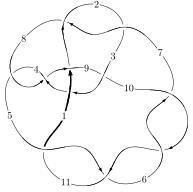
\includegraphics[width=112pt]{../../../GIT/diagram.site/Diagrams/png/594_11a_345.png}\\
\ \ \ A knot diagram\footnotemark}&
\allowdisplaybreaks
\textbf{Linearized knot diagam} \\
\cline{2-2}
 &
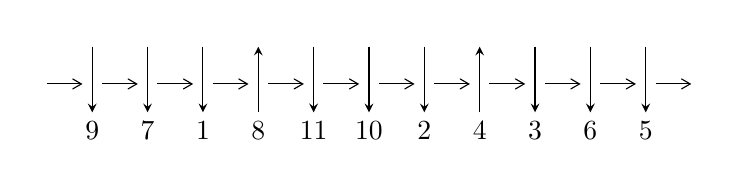
\begin{tikzpicture}[x=20pt, y=17pt]
	% nodes
	\node (C0) at (0, 0) {};
	\node (C1) at (1, 0) {};
	\node (C1U) at (1, +1) {};
	\node (C1D) at (1, -1) {9};

	\node (C2) at (2, 0) {};
	\node (C2U) at (2, +1) {};
	\node (C2D) at (2, -1) {7};

	\node (C3) at (3, 0) {};
	\node (C3U) at (3, +1) {};
	\node (C3D) at (3, -1) {1};

	\node (C4) at (4, 0) {};
	\node (C4U) at (4, +1) {};
	\node (C4D) at (4, -1) {8};

	\node (C5) at (5, 0) {};
	\node (C5U) at (5, +1) {};
	\node (C5D) at (5, -1) {11};

	\node (C6) at (6, 0) {};
	\node (C6U) at (6, +1) {};
	\node (C6D) at (6, -1) {10};

	\node (C7) at (7, 0) {};
	\node (C7U) at (7, +1) {};
	\node (C7D) at (7, -1) {2};

	\node (C8) at (8, 0) {};
	\node (C8U) at (8, +1) {};
	\node (C8D) at (8, -1) {4};

	\node (C9) at (9, 0) {};
	\node (C9U) at (9, +1) {};
	\node (C9D) at (9, -1) {3};

	\node (C10) at (10, 0) {};
	\node (C10U) at (10, +1) {};
	\node (C10D) at (10, -1) {6};

	\node (C11) at (11, 0) {};
	\node (C11U) at (11, +1) {};
	\node (C11D) at (11, -1) {5};
	\node (C12) at (12, 0) {};

	% arrows
	\draw[->,>={angle 60}]
	(C0) edge (C1) (C1) edge (C2) (C2) edge (C3) (C3) edge (C4) (C4) edge (C5) (C5) edge (C6) (C6) edge (C7) (C7) edge (C8) (C8) edge (C9) (C9) edge (C10) (C10) edge (C11) (C11) edge (C12) ;	\draw[->,>=stealth]
	(C1U) edge (C1D) (C2U) edge (C2D) (C3U) edge (C3D) (C4D) edge (C4U) (C5U) edge (C5D) (C6U) edge (C6D) (C7U) edge (C7D) (C8D) edge (C8U) (C9U) edge (C9D) (C10U) edge (C10D) (C11U) edge (C11D) ;
	\end{tikzpicture} \\
\hhline{~~} \\& 
\textbf{Solving Sequence} \\ \cline{2-2} 
 &
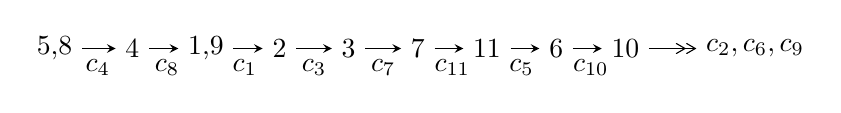
\begin{tikzpicture}[x=25pt, y=7pt]
	% node
	\node (A0) at (-1/8, 0) {5,8};
	\node (A1) at (1, 0) {4};
	\node (A2) at (33/16, 0) {1,9};
	\node (A3) at (25/8, 0) {2};
	\node (A4) at (33/8, 0) {3};
	\node (A5) at (41/8, 0) {7};
	\node (A6) at (49/8, 0) {11};
	\node (A7) at (57/8, 0) {6};
	\node (A8) at (65/8, 0) {10};
	\node (C1) at (1/2, -1) {$c_{4}$};
	\node (C2) at (3/2, -1) {$c_{8}$};
	\node (C3) at (21/8, -1) {$c_{1}$};
	\node (C4) at (29/8, -1) {$c_{3}$};
	\node (C5) at (37/8, -1) {$c_{7}$};
	\node (C6) at (45/8, -1) {$c_{11}$};
	\node (C7) at (53/8, -1) {$c_{5}$};
	\node (C8) at (61/8, -1) {$c_{10}$};
	\node (A9) at (10, 0) {$c_{2},c_{6},c_{9}$};

	% edge
	\draw[->,>=stealth]	
	(A0) edge (A1) (A1) edge (A2) (A2) edge (A3) (A3) edge (A4) (A4) edge (A5) (A5) edge (A6) (A6) edge (A7) (A7) edge (A8) ;
	\draw[->>,>={angle 60}]	
	(A8) edge (A9);
\end{tikzpicture} \\ 

\end{tabular} \\

\footnotetext{
The image of knot diagram is generated by the software ``\textbf{Draw programme}" developed by Andrew Bartholomew(\url{http://www.layer8.co.uk/maths/draw/index.htm\#Running-draw}), where we modified some parts for our purpose(\url{https://github.com/CATsTAILs/LinksPainter}).
}\phantom \\ \newline 
\centering \textbf{Ideals for irreducible components\footnotemark of $X_{\text{par}}$} 
 
\begin{align*}
I^u_{1}&=\langle 
-1.06878\times10^{64} u^{54}-1.33106\times10^{64} u^{53}+\cdots+2.34911\times10^{64} b+3.10634\times10^{65},\\
\phantom{I^u_{1}}&\phantom{= \langle  }-4.96423\times10^{64} u^{54}-3.38365\times10^{65} u^{53}+\cdots+4.46331\times10^{65} a+4.84254\times10^{66},\\
\phantom{I^u_{1}}&\phantom{= \langle  }u^{55}+2 u^{54}+\cdots-21 u-19\rangle \\
I^u_{2}&=\langle 
- u^9-2 u^7-3 u^6-4 u^5-7 u^4- u^3-10 u^2+b-3,\\
\phantom{I^u_{2}}&\phantom{= \langle  }u^9-2 u^8+4 u^7-5 u^6+8 u^5-11 u^4+7 u^3-9 u^2+a+2 u-5,\\
\phantom{I^u_{2}}&\phantom{= \langle  }u^{10}- u^9+4 u^8-2 u^7+9 u^6-3 u^5+10 u^4- u^3+5 u^2+1\rangle \\
\\
\end{align*}
\raggedright * 2 irreducible components of $\dim_{\mathbb{C}}=0$, with total 65 representations.\\
\footnotetext{All coefficients of polynomials are rational numbers. But the coefficients are sometimes approximated in decimal forms when there is not enough margin.}
\newpage
\renewcommand{\arraystretch}{1}
\centering \section*{I. $I^u_{1}= \langle -1.07\times10^{64} u^{54}-1.33\times10^{64} u^{53}+\cdots+2.35\times10^{64} b+3.11\times10^{65},\;-4.96\times10^{64} u^{54}-3.38\times10^{65} u^{53}+\cdots+4.46\times10^{65} a+4.84\times10^{66},\;u^{55}+2 u^{54}+\cdots-21 u-19 \rangle$}
\flushleft \textbf{(i) Arc colorings}\\
\begin{tabular}{m{7pt} m{180pt} m{7pt} m{180pt} }
\flushright $a_{5}=$&$\begin{pmatrix}1\\0\end{pmatrix}$ \\
\flushright $a_{8}=$&$\begin{pmatrix}0\\u\end{pmatrix}$ \\
\flushright $a_{4}=$&$\begin{pmatrix}1\\u^2\end{pmatrix}$ \\
\flushright $a_{1}=$&$\begin{pmatrix}0.111223 u^{54}+0.758104 u^{53}+\cdots-2.14133 u-10.8497\\0.454971 u^{54}+0.566623 u^{53}+\cdots+0.405867 u-13.2235\end{pmatrix}$ \\
\flushright $a_{9}=$&$\begin{pmatrix}u\\u^3+u\end{pmatrix}$ \\
\flushright $a_{2}=$&$\begin{pmatrix}0.237528 u^{54}+0.475907 u^{53}+\cdots-8.87677 u-2.80560\\0.821183 u^{54}+1.24967 u^{53}+\cdots-15.1607 u-15.3408\end{pmatrix}$ \\
\flushright $a_{3}=$&$\begin{pmatrix}-0.203904 u^{54}+1.47436 u^{53}+\cdots+12.2860 u-39.9386\\-0.967112 u^{54}-1.05043 u^{53}+\cdots+16.7082 u-2.90059\end{pmatrix}$ \\
\flushright $a_{7}=$&$\begin{pmatrix}-1.45501 u^{54}-2.10564 u^{53}+\cdots+32.3133 u+9.63822\\-0.567890 u^{54}-1.35518 u^{53}+\cdots+23.9697 u+10.6270\end{pmatrix}$ \\
\flushright $a_{11}=$&$\begin{pmatrix}0.566195 u^{54}+1.32473 u^{53}+\cdots-1.73546 u-24.0732\\0.454971 u^{54}+0.566623 u^{53}+\cdots+0.405867 u-13.2235\end{pmatrix}$ \\
\flushright $a_{6}=$&$\begin{pmatrix}1.49742 u^{54}+2.39469 u^{53}+\cdots-43.4290 u-0.564570\\0.356541 u^{54}+0.824208 u^{53}+\cdots-9.96821 u-10.6136\end{pmatrix}$ \\
\flushright $a_{10}=$&$\begin{pmatrix}-0.0874572 u^{54}-1.59572 u^{53}+\cdots+35.1757 u+23.3627\\-0.419464 u^{54}-0.762736 u^{53}+\cdots+15.0261 u+9.25174\end{pmatrix}$\\ \flushright $a_{10}=$&$\begin{pmatrix}-0.0874572 u^{54}-1.59572 u^{53}+\cdots+35.1757 u+23.3627\\-0.419464 u^{54}-0.762736 u^{53}+\cdots+15.0261 u+9.25174\end{pmatrix}$\\&\end{tabular}
\flushleft \textbf{(ii) Obstruction class $= -1$}\\~\\
\flushleft \textbf{(iii) Cusp Shapes $= 2.37110 u^{54}+5.51320 u^{53}+\cdots-14.4173 u-120.988$}\\~\\
\newpage\renewcommand{\arraystretch}{1}
\flushleft \textbf{(iv) u-Polynomials at the component}\newline \\
\begin{tabular}{m{50pt}|m{274pt}}
Crossings & \hspace{64pt}u-Polynomials at each crossing \\
\hline $$\begin{aligned}c_{1}\end{aligned}$$&$\begin{aligned}
&u^{55}+3 u^{54}+\cdots+3 u^2+1
\end{aligned}$\\
\hline $$\begin{aligned}c_{2},c_{7}\end{aligned}$$&$\begin{aligned}
&u^{55}- u^{54}+\cdots-8 u+88
\end{aligned}$\\
\hline $$\begin{aligned}c_{3}\end{aligned}$$&$\begin{aligned}
&u^{55}-9 u^{54}+\cdots-76 u+7
\end{aligned}$\\
\hline $$\begin{aligned}c_{4},c_{8}\end{aligned}$$&$\begin{aligned}
&u^{55}-2 u^{54}+\cdots-21 u+19
\end{aligned}$\\
\hline $$\begin{aligned}c_{5},c_{6},c_{10}\\c_{11}\end{aligned}$$&$\begin{aligned}
&u^{55}+u^{54}+\cdots-5 u+7
\end{aligned}$\\
\hline $$\begin{aligned}c_{9}\end{aligned}$$&$\begin{aligned}
&u^{55}+12 u^{53}+\cdots-2271 u+6677
\end{aligned}$\\
\hline
\end{tabular}\\~\\
\newpage\renewcommand{\arraystretch}{1}
\flushleft \textbf{(v) Riley Polynomials at the component}\newline \\
\begin{tabular}{m{50pt}|m{274pt}}
Crossings & \hspace{64pt}Riley Polynomials at each crossing \\
\hline $$\begin{aligned}c_{1}\end{aligned}$$&$\begin{aligned}
&y^{55}-3 y^{54}+\cdots-6 y-1
\end{aligned}$\\
\hline $$\begin{aligned}c_{2},c_{7}\end{aligned}$$&$\begin{aligned}
&y^{55}+45 y^{54}+\cdots-134048 y-7744
\end{aligned}$\\
\hline $$\begin{aligned}c_{3}\end{aligned}$$&$\begin{aligned}
&y^{55}+3 y^{54}+\cdots-160 y-49
\end{aligned}$\\
\hline $$\begin{aligned}c_{4},c_{8}\end{aligned}$$&$\begin{aligned}
&y^{55}+30 y^{54}+\cdots-927 y-361
\end{aligned}$\\
\hline $$\begin{aligned}c_{5},c_{6},c_{10}\\c_{11}\end{aligned}$$&$\begin{aligned}
&y^{55}+69 y^{54}+\cdots-843 y-49
\end{aligned}$\\
\hline $$\begin{aligned}c_{9}\end{aligned}$$&$\begin{aligned}
&y^{55}+24 y^{54}+\cdots-671436323 y-44582329
\end{aligned}$\\
\hline
\end{tabular}\\~\\
\newpage\flushleft \textbf{(vi) Complex Volumes and Cusp Shapes}
$$\begin{array}{c|c|c}  
\text{Solutions to }I^u_{1}& \I (\text{vol} + \sqrt{-1}CS) & \text{Cusp shape}\\
 \hline 
\begin{aligned}
u &= -0.401482 + 0.925485 I \\
a &= -2.81752 - 0.40677 I \\
b &= -0.01279 + 1.63475 I\end{aligned}
 & \phantom{-}12.00640 + 0.63513 I & -0.597872 + 0.536133 I \\ \hline\begin{aligned}
u &= -0.401482 - 0.925485 I \\
a &= -2.81752 + 0.40677 I \\
b &= -0.01279 - 1.63475 I\end{aligned}
 & \phantom{-}12.00640 - 0.63513 I & -0.597872 - 0.536133 I \\ \hline\begin{aligned}
u &= -0.476583 + 0.910485 I \\
a &= \phantom{-}2.02609 + 0.84809 I \\
b &= -0.19570 - 1.65977 I\end{aligned}
 & \phantom{-}12.54410 - 5.30776 I & -0.93873 + 5.45617 I \\ \hline\begin{aligned}
u &= -0.476583 - 0.910485 I \\
a &= \phantom{-}2.02609 - 0.84809 I \\
b &= -0.19570 + 1.65977 I\end{aligned}
 & \phantom{-}12.54410 + 5.30776 I & -0.93873 - 5.45617 I \\ \hline\begin{aligned}
u &= \phantom{-}0.312846 + 0.902609 I \\
a &= -0.594280 - 0.941337 I \\
b &= \phantom{-}0.140808 - 0.966052 I\end{aligned}
 & \phantom{-}3.17927 + 3.14967 I & -1.09390 - 6.92052 I \\ \hline\begin{aligned}
u &= \phantom{-}0.312846 - 0.902609 I \\
a &= -0.594280 + 0.941337 I \\
b &= \phantom{-}0.140808 + 0.966052 I\end{aligned}
 & \phantom{-}3.17927 - 3.14967 I & -1.09390 + 6.92052 I \\ \hline\begin{aligned}
u &= \phantom{-}0.415600 + 0.985014 I \\
a &= -0.590021 - 0.574831 I \\
b &= \phantom{-}0.610435 + 1.043970 I\end{aligned}
 & \phantom{-}3.21288 + 1.41327 I & -0.79892 - 2.47902 I \\ \hline\begin{aligned}
u &= \phantom{-}0.415600 - 0.985014 I \\
a &= -0.590021 + 0.574831 I \\
b &= \phantom{-}0.610435 - 1.043970 I\end{aligned}
 & \phantom{-}3.21288 - 1.41327 I & -0.79892 + 2.47902 I \\ \hline\begin{aligned}
u &= \phantom{-}0.912208 + 0.038959 I \\
a &= -0.394969 + 0.552527 I \\
b &= \phantom{-}0.02833 + 1.64604 I\end{aligned}
 & \phantom{-}10.07850 - 2.31202 I & -1.07799 + 2.78280 I \\ \hline\begin{aligned}
u &= \phantom{-}0.912208 - 0.038959 I \\
a &= -0.394969 - 0.552527 I \\
b &= \phantom{-}0.02833 - 1.64604 I\end{aligned}
 & \phantom{-}10.07850 + 2.31202 I & -1.07799 - 2.78280 I\\
 \hline 
 \end{array}$$\newpage$$\begin{array}{c|c|c}  
\text{Solutions to }I^u_{1}& \I (\text{vol} + \sqrt{-1}CS) & \text{Cusp shape}\\
 \hline 
\begin{aligned}
u &= \phantom{-}0.311945 + 1.050300 I \\
a &= \phantom{-}1.362230 + 0.285561 I \\
b &= -0.518495 - 0.178316 I\end{aligned}
 & -3.26165 + 2.54833 I & -12.38074 + 0. I\phantom{ +0.000000I} \\ \hline\begin{aligned}
u &= \phantom{-}0.311945 - 1.050300 I \\
a &= \phantom{-}1.362230 - 0.285561 I \\
b &= -0.518495 + 0.178316 I\end{aligned}
 & -3.26165 - 2.54833 I & -12.38074 + 0. I\phantom{ +0.000000I} \\ \hline\begin{aligned}
u &= \phantom{-}1.061010 + 0.282738 I \\
a &= \phantom{-}0.149658 - 0.140466 I \\
b &= -0.420813 - 0.866276 I\end{aligned}
 & \phantom{-}5.77965 - 5.30825 I & \phantom{-0.000000 -}0. + 6.19930 I \\ \hline\begin{aligned}
u &= \phantom{-}1.061010 - 0.282738 I \\
a &= \phantom{-}0.149658 + 0.140466 I \\
b &= -0.420813 + 0.866276 I\end{aligned}
 & \phantom{-}5.77965 + 5.30825 I & \phantom{-0.000000 } 0. - 6.19930 I \\ \hline\begin{aligned}
u &= -0.071907 + 0.862619 I \\
a &= \phantom{-}1.13431 - 0.98072 I \\
b &= -0.178670 + 1.238420 I\end{aligned}
 & \phantom{-}1.097690 - 0.148579 I & -6.50751 - 0.03024 I \\ \hline\begin{aligned}
u &= -0.071907 - 0.862619 I \\
a &= \phantom{-}1.13431 + 0.98072 I \\
b &= -0.178670 - 1.238420 I\end{aligned}
 & \phantom{-}1.097690 + 0.148579 I & -6.50751 + 0.03024 I \\ \hline\begin{aligned}
u &= -0.444288 + 0.734086 I \\
a &= \phantom{-}0.286988 + 0.144362 I \\
b &= \phantom{-}0.12278 - 1.74080 I\end{aligned}
 & \phantom{-}13.12830 + 1.45980 I & -0.69339 + 1.95269 I \\ \hline\begin{aligned}
u &= -0.444288 - 0.734086 I \\
a &= \phantom{-}0.286988 - 0.144362 I \\
b &= \phantom{-}0.12278 + 1.74080 I\end{aligned}
 & \phantom{-}13.12830 - 1.45980 I & -0.69339 - 1.95269 I \\ \hline\begin{aligned}
u &= -0.326526 + 1.106980 I \\
a &= -0.974994 + 0.074120 I \\
b &= \phantom{-}0.472889 + 0.479834 I\end{aligned}
 & -1.01300 - 1.69462 I & \phantom{-0.000000 } 0 \\ \hline\begin{aligned}
u &= -0.326526 - 1.106980 I \\
a &= -0.974994 - 0.074120 I \\
b &= \phantom{-}0.472889 - 0.479834 I\end{aligned}
 & -1.01300 + 1.69462 I & \phantom{-0.000000 } 0\\
 \hline 
 \end{array}$$\newpage$$\begin{array}{c|c|c}  
\text{Solutions to }I^u_{1}& \I (\text{vol} + \sqrt{-1}CS) & \text{Cusp shape}\\
 \hline 
\begin{aligned}
u &= -0.345937 + 0.758860 I \\
a &= -0.84685 + 1.65125 I \\
b &= \phantom{-}0.04042 + 1.69986 I\end{aligned}
 & \phantom{-}12.61370 - 3.89122 I & -0.20719 + 8.96757 I \\ \hline\begin{aligned}
u &= -0.345937 - 0.758860 I \\
a &= -0.84685 - 1.65125 I \\
b &= \phantom{-}0.04042 - 1.69986 I\end{aligned}
 & \phantom{-}12.61370 + 3.89122 I & -0.20719 - 8.96757 I \\ \hline\begin{aligned}
u &= -0.070037 + 1.186880 I \\
a &= -0.772712 - 0.062250 I \\
b &= \phantom{-}0.456547 + 0.410612 I\end{aligned}
 & -1.14656 - 1.61384 I & \phantom{-0.000000 } 0 \\ \hline\begin{aligned}
u &= -0.070037 - 1.186880 I \\
a &= -0.772712 + 0.062250 I \\
b &= \phantom{-}0.456547 - 0.410612 I\end{aligned}
 & -1.14656 + 1.61384 I & \phantom{-0.000000 } 0 \\ \hline\begin{aligned}
u &= \phantom{-}0.262970 + 0.735642 I \\
a &= -2.80343 + 0.00413 I \\
b &= -0.073778 - 0.672365 I\end{aligned}
 & \phantom{-}3.83511 - 0.35945 I & -0.43782 - 1.63118 I \\ \hline\begin{aligned}
u &= \phantom{-}0.262970 - 0.735642 I \\
a &= -2.80343 - 0.00413 I \\
b &= -0.073778 + 0.672365 I\end{aligned}
 & \phantom{-}3.83511 + 0.35945 I & -0.43782 + 1.63118 I \\ \hline\begin{aligned}
u &= -0.427599 + 1.157360 I \\
a &= \phantom{-}1.55960 + 0.23930 I \\
b &= -0.371626 - 0.726720 I\end{aligned}
 & -1.61640 - 5.63449 I & \phantom{-0.000000 } 0 \\ \hline\begin{aligned}
u &= -0.427599 - 1.157360 I \\
a &= \phantom{-}1.55960 - 0.23930 I \\
b &= -0.371626 + 0.726720 I\end{aligned}
 & -1.61640 + 5.63449 I & \phantom{-0.000000 } 0 \\ \hline\begin{aligned}
u &= -0.499880 + 1.150480 I \\
a &= -1.164720 + 0.331774 I \\
b &= \phantom{-}0.864118 - 0.012965 I\end{aligned}
 & \phantom{-}0.07105 - 6.42965 I & \phantom{-0.000000 } 0 \\ \hline\begin{aligned}
u &= -0.499880 - 1.150480 I \\
a &= -1.164720 - 0.331774 I \\
b &= \phantom{-}0.864118 + 0.012965 I\end{aligned}
 & \phantom{-}0.07105 + 6.42965 I & \phantom{-0.000000 } 0\\
 \hline 
 \end{array}$$\newpage$$\begin{array}{c|c|c}  
\text{Solutions to }I^u_{1}& \I (\text{vol} + \sqrt{-1}CS) & \text{Cusp shape}\\
 \hline 
\begin{aligned}
u &= \phantom{-}0.364876 + 0.632638 I \\
a &= \phantom{-}2.34792 - 0.06805 I \\
b &= -0.645292 + 0.720286 I\end{aligned}
 & \phantom{-}4.35568 + 2.03916 I & \phantom{-}0.91927 - 6.28505 I \\ \hline\begin{aligned}
u &= \phantom{-}0.364876 - 0.632638 I \\
a &= \phantom{-}2.34792 + 0.06805 I \\
b &= -0.645292 - 0.720286 I\end{aligned}
 & \phantom{-}4.35568 - 2.03916 I & \phantom{-}0.91927 + 6.28505 I \\ \hline\begin{aligned}
u &= -0.710497 + 0.126727 I \\
a &= \phantom{-}0.289263 - 0.813765 I \\
b &= -0.583790 + 0.094289 I\end{aligned}
 & \phantom{-}2.94002 + 1.90835 I & -3.01939 - 3.01750 I \\ \hline\begin{aligned}
u &= -0.710497 - 0.126727 I \\
a &= \phantom{-}0.289263 + 0.813765 I \\
b &= -0.583790 - 0.094289 I\end{aligned}
 & \phantom{-}2.94002 - 1.90835 I & -3.01939 + 3.01750 I \\ \hline\begin{aligned}
u &= -0.515161 + 1.175820 I \\
a &= \phantom{-}0.243302 - 0.148831 I \\
b &= -0.118294 + 0.339429 I\end{aligned}
 & -1.10271 - 2.46020 I & \phantom{-0.000000 } 0 \\ \hline\begin{aligned}
u &= -0.515161 - 1.175820 I \\
a &= \phantom{-}0.243302 + 0.148831 I \\
b &= -0.118294 - 0.339429 I\end{aligned}
 & -1.10271 + 2.46020 I & \phantom{-0.000000 } 0 \\ \hline\begin{aligned}
u &= -1.234950 + 0.406378 I \\
a &= \phantom{-}0.056972 + 0.536788 I \\
b &= -0.12025 + 1.66551 I\end{aligned}
 & \phantom{-}14.5361 + 7.4191 I & \phantom{-0.000000 } 0 \\ \hline\begin{aligned}
u &= -1.234950 - 0.406378 I \\
a &= \phantom{-}0.056972 - 0.536788 I \\
b &= -0.12025 - 1.66551 I\end{aligned}
 & \phantom{-}14.5361 - 7.4191 I & \phantom{-0.000000 } 0 \\ \hline\begin{aligned}
u &= \phantom{-}0.511227 + 1.223850 I \\
a &= \phantom{-}1.80919 - 0.59265 I \\
b &= -0.09200 + 1.63412 I\end{aligned}
 & \phantom{-}6.56631 + 7.31158 I & \phantom{-0.000000 } 0 \\ \hline\begin{aligned}
u &= \phantom{-}0.511227 - 1.223850 I \\
a &= \phantom{-}1.80919 + 0.59265 I \\
b &= -0.09200 - 1.63412 I\end{aligned}
 & \phantom{-}6.56631 - 7.31158 I & \phantom{-0.000000 } 0\\
 \hline 
 \end{array}$$\newpage$$\begin{array}{c|c|c}  
\text{Solutions to }I^u_{1}& \I (\text{vol} + \sqrt{-1}CS) & \text{Cusp shape}\\
 \hline 
\begin{aligned}
u &= \phantom{-}0.615900 + 1.225140 I \\
a &= -1.385260 - 0.069629 I \\
b &= \phantom{-}0.588670 - 0.914922 I\end{aligned}
 & \phantom{-}2.82511 + 11.22660 I & \phantom{-0.000000 } 0 \\ \hline\begin{aligned}
u &= \phantom{-}0.615900 - 1.225140 I \\
a &= -1.385260 + 0.069629 I \\
b &= \phantom{-}0.588670 + 0.914922 I\end{aligned}
 & \phantom{-}2.82511 - 11.22660 I & \phantom{-0.000000 } 0 \\ \hline\begin{aligned}
u &= \phantom{-}0.817752 + 1.114980 I \\
a &= \phantom{-}0.672880 + 0.363392 I \\
b &= -0.117271 + 0.670556 I\end{aligned}
 & -0.18164 + 3.45397 I & \phantom{-0.000000 } 0 \\ \hline\begin{aligned}
u &= \phantom{-}0.817752 - 1.114980 I \\
a &= \phantom{-}0.672880 - 0.363392 I \\
b &= -0.117271 - 0.670556 I\end{aligned}
 & -0.18164 - 3.45397 I & \phantom{-0.000000 } 0 \\ \hline\begin{aligned}
u &= -0.615666 + 0.002465 I \\
a &= -0.603564 - 0.058474 I \\
b &= \phantom{-}0.151090 - 0.780801 I\end{aligned}
 & \phantom{-}1.58788 + 1.71112 I & -2.31712 - 4.70415 I \\ \hline\begin{aligned}
u &= -0.615666 - 0.002465 I \\
a &= -0.603564 + 0.058474 I \\
b &= \phantom{-}0.151090 + 0.780801 I\end{aligned}
 & \phantom{-}1.58788 - 1.71112 I & -2.31712 + 4.70415 I \\ \hline\begin{aligned}
u &= \phantom{-}0.780839 + 1.175860 I \\
a &= -0.977962 - 0.072520 I \\
b &= \phantom{-}0.11048 - 1.52706 I\end{aligned}
 & \phantom{-}5.67173 + 3.68365 I & \phantom{-0.000000 } 0 \\ \hline\begin{aligned}
u &= \phantom{-}0.780839 - 1.175860 I \\
a &= -0.977962 + 0.072520 I \\
b &= \phantom{-}0.11048 + 1.52706 I\end{aligned}
 & \phantom{-}5.67173 - 3.68365 I & \phantom{-0.000000 } 0 \\ \hline\begin{aligned}
u &= -0.71320 + 1.26334 I \\
a &= -1.53597 - 0.11861 I \\
b &= \phantom{-}0.17113 + 1.68532 I\end{aligned}
 & \phantom{-}11.7421 - 14.2160 I & \phantom{-0.000000 } 0 \\ \hline\begin{aligned}
u &= -0.71320 - 1.26334 I \\
a &= -1.53597 + 0.11861 I \\
b &= \phantom{-}0.17113 - 1.68532 I\end{aligned}
 & \phantom{-}11.7421 + 14.2160 I & \phantom{-0.000000 } 0\\
 \hline 
 \end{array}$$\newpage$$\begin{array}{c|c|c}  
\text{Solutions to }I^u_{1}& \I (\text{vol} + \sqrt{-1}CS) & \text{Cusp shape}\\
 \hline 
\begin{aligned}
u &= \phantom{-}0.32406 + 1.47876 I \\
a &= -0.398309 + 0.645182 I \\
b &= \phantom{-}0.04652 - 1.56492 I\end{aligned}
 & \phantom{-}5.43122 + 2.80843 I & \phantom{-0.000000 } 0 \\ \hline\begin{aligned}
u &= \phantom{-}0.32406 - 1.47876 I \\
a &= -0.398309 - 0.645182 I \\
b &= \phantom{-}0.04652 + 1.56492 I\end{aligned}
 & \phantom{-}5.43122 - 2.80843 I & \phantom{-0.000000 } 0 \\ \hline\begin{aligned}
u &= -0.99875 + 1.14713 I \\
a &= \phantom{-}0.882856 - 0.413980 I \\
b &= -0.02860 - 1.62809 I\end{aligned}
 & \phantom{-}7.90755 - 3.97377 I & \phantom{-0.000000 } 0 \\ \hline\begin{aligned}
u &= -0.99875 - 1.14713 I \\
a &= \phantom{-}0.882856 + 0.413980 I \\
b &= -0.02860 + 1.62809 I\end{aligned}
 & \phantom{-}7.90755 + 3.97377 I & \phantom{-0.000000 } 0 \\ \hline\begin{aligned}
u &= \phantom{-}0.322466\phantom{ +0.000000I} \\
a &= -1.13192\phantom{ +0.000000I} \\
b &= \phantom{-}0.346289\phantom{ +0.000000I}\end{aligned}
 & -0.742548\phantom{ +0.000000I} & -13.8050\phantom{ +0.000000I}\\
 \hline 
 \end{array}$$\newpage\newpage\renewcommand{\arraystretch}{1}
\centering \section*{II. $I^u_{2}= \langle - u^9-2 u^7+\cdots+b-3,\;u^9-2 u^8+\cdots+a-5,\;u^{10}- u^9+\cdots+5 u^2+1 \rangle$}
\flushleft \textbf{(i) Arc colorings}\\
\begin{tabular}{m{7pt} m{180pt} m{7pt} m{180pt} }
\flushright $a_{5}=$&$\begin{pmatrix}1\\0\end{pmatrix}$ \\
\flushright $a_{8}=$&$\begin{pmatrix}0\\u\end{pmatrix}$ \\
\flushright $a_{4}=$&$\begin{pmatrix}1\\u^2\end{pmatrix}$ \\
\flushright $a_{1}=$&$\begin{pmatrix}- u^9+2 u^8-4 u^7+5 u^6-8 u^5+11 u^4-7 u^3+9 u^2-2 u+5\\u^9+2 u^7+3 u^6+4 u^5+7 u^4+u^3+10 u^2+3\end{pmatrix}$ \\
\flushright $a_{9}=$&$\begin{pmatrix}u\\u^3+u\end{pmatrix}$ \\
\flushright $a_{2}=$&$\begin{pmatrix}u^8- u^7+4 u^6-2 u^5+9 u^4-3 u^3+10 u^2- u+5\\u^9+2 u^7+3 u^6+4 u^5+7 u^4+u^3+11 u^2+3\end{pmatrix}$ \\
\flushright $a_{3}=$&$\begin{pmatrix}u^9-5 u^8+8 u^7-17 u^6+16 u^5-35 u^4+20 u^3-32 u^2+6 u-10\\u^9-3 u^8+6 u^7-9 u^6+12 u^5-17 u^4+14 u^3-12 u^2+4 u-2\end{pmatrix}$ \\
\flushright $a_{7}=$&$\begin{pmatrix}5 u^9-5 u^8+19 u^7-9 u^6+41 u^5-13 u^4+41 u^3-2 u^2+15 u+1\\3 u^9-4 u^8+12 u^7-8 u^6+24 u^5-13 u^4+23 u^3-4 u^2+5 u\end{pmatrix}$ \\
\flushright $a_{11}=$&$\begin{pmatrix}2 u^8-2 u^7+8 u^6-4 u^5+18 u^4-6 u^3+19 u^2-2 u+8\\u^9+2 u^7+3 u^6+4 u^5+7 u^4+u^3+10 u^2+3\end{pmatrix}$ \\
\flushright $a_{6}=$&$\begin{pmatrix}- u^9+5 u^8-9 u^7+17 u^6-18 u^5+33 u^4-24 u^3+28 u^2-7 u+6\\-3 u^9+3 u^8-11 u^7+5 u^6-23 u^5+7 u^4-21 u^3-6 u-2\end{pmatrix}$ \\
\flushright $a_{10}=$&$\begin{pmatrix}-6 u^9+5 u^8-20 u^7+5 u^6-41 u^5+4 u^4-34 u^3-11 u^2-7 u-5\\- u^8+2 u^7-5 u^6+5 u^5-10 u^4+9 u^3-11 u^2+5 u-3\end{pmatrix}$\\ \flushright $a_{10}=$&$\begin{pmatrix}-6 u^9+5 u^8-20 u^7+5 u^6-41 u^5+4 u^4-34 u^3-11 u^2-7 u-5\\- u^8+2 u^7-5 u^6+5 u^5-10 u^4+9 u^3-11 u^2+5 u-3\end{pmatrix}$\\&\end{tabular}
\flushleft \textbf{(ii) Obstruction class $= 1$}\\~\\
\flushleft \textbf{(iii) Cusp Shapes $= u^9-4 u^8+7 u^7-12 u^6+12 u^5-21 u^4+13 u^3-18 u^2-9$}\\~\\
\newpage\renewcommand{\arraystretch}{1}
\flushleft \textbf{(iv) u-Polynomials at the component}\newline \\
\begin{tabular}{m{50pt}|m{274pt}}
Crossings & \hspace{64pt}u-Polynomials at each crossing \\
\hline $$\begin{aligned}c_{1}\end{aligned}$$&$\begin{aligned}
&u^{10}-2 u^9+u^8- u^6- u^5+3 u^4+u^3- u^2- u+1
\end{aligned}$\\
\hline $$\begin{aligned}c_{2}\end{aligned}$$&$\begin{aligned}
&u^{10}+5 u^8+u^7+10 u^6+3 u^5+9 u^4+2 u^3+4 u^2+u+1
\end{aligned}$\\
\hline $$\begin{aligned}c_{3}\end{aligned}$$&$\begin{aligned}
&u^{10}+3 u^7+3 u^6-2 u^5-3 u^4+u^3+4 u^2+3 u+1
\end{aligned}$\\
\hline $$\begin{aligned}c_{4}\end{aligned}$$&$\begin{aligned}
&u^{10}- u^9+4 u^8-2 u^7+9 u^6-3 u^5+10 u^4- u^3+5 u^2+1
\end{aligned}$\\
\hline $$\begin{aligned}c_{5},c_{6}\end{aligned}$$&$\begin{aligned}
&u^{10}+7 u^8+17 u^6+17 u^4- u^3+7 u^2-2 u+1
\end{aligned}$\\
\hline $$\begin{aligned}c_{7}\end{aligned}$$&$\begin{aligned}
&u^{10}+5 u^8- u^7+10 u^6-3 u^5+9 u^4-2 u^3+4 u^2- u+1
\end{aligned}$\\
\hline $$\begin{aligned}c_{8}\end{aligned}$$&$\begin{aligned}
&u^{10}+u^9+4 u^8+2 u^7+9 u^6+3 u^5+10 u^4+u^3+5 u^2+1
\end{aligned}$\\
\hline $$\begin{aligned}c_{9}\end{aligned}$$&$\begin{aligned}
&u^{10}+u^9- u^8- u^7+3 u^6+u^5- u^4+u^2+2 u+1
\end{aligned}$\\
\hline $$\begin{aligned}c_{10},c_{11}\end{aligned}$$&$\begin{aligned}
&u^{10}+7 u^8+17 u^6+17 u^4+u^3+7 u^2+2 u+1
\end{aligned}$\\
\hline
\end{tabular}\\~\\
\newpage\renewcommand{\arraystretch}{1}
\flushleft \textbf{(v) Riley Polynomials at the component}\newline \\
\begin{tabular}{m{50pt}|m{274pt}}
Crossings & \hspace{64pt}Riley Polynomials at each crossing \\
\hline $$\begin{aligned}c_{1}\end{aligned}$$&$\begin{aligned}
&y^{10}-2 y^9- y^8+9 y^6-11 y^5+15 y^4-11 y^3+9 y^2-3 y+1
\end{aligned}$\\
\hline $$\begin{aligned}c_{2},c_{7}\end{aligned}$$&$\begin{aligned}
&y^{10}+10 y^9+\cdots+7 y+1
\end{aligned}$\\
\hline $$\begin{aligned}c_{3}\end{aligned}$$&$\begin{aligned}
&y^{10}+6 y^8-15 y^7+29 y^6-26 y^5+19 y^4-7 y^3+4 y^2- y+1
\end{aligned}$\\
\hline $$\begin{aligned}c_{4},c_{8}\end{aligned}$$&$\begin{aligned}
&y^{10}+7 y^9+\cdots+10 y+1
\end{aligned}$\\
\hline $$\begin{aligned}c_{5},c_{6},c_{10}\\c_{11}\end{aligned}$$&$\begin{aligned}
&y^{10}+14 y^9+\cdots+10 y+1
\end{aligned}$\\
\hline $$\begin{aligned}c_{9}\end{aligned}$$&$\begin{aligned}
&y^{10}-3 y^9+9 y^8-11 y^7+15 y^6-11 y^5+9 y^4- y^2-2 y+1
\end{aligned}$\\
\hline
\end{tabular}\\~\\
\newpage\flushleft \textbf{(vi) Complex Volumes and Cusp Shapes}
$$\begin{array}{c|c|c}  
\text{Solutions to }I^u_{2}& \I (\text{vol} + \sqrt{-1}CS) & \text{Cusp shape}\\
 \hline 
\begin{aligned}
u &= \phantom{-}0.376339 + 0.979659 I \\
a &= -0.010197 - 0.670492 I \\
b &= \phantom{-}0.177185 + 1.148900 I\end{aligned}
 & \phantom{-}1.42305 + 1.66512 I & -4.81318 - 3.74793 I \\ \hline\begin{aligned}
u &= \phantom{-}0.376339 - 0.979659 I \\
a &= -0.010197 + 0.670492 I \\
b &= \phantom{-}0.177185 - 1.148900 I\end{aligned}
 & \phantom{-}1.42305 - 1.66512 I & -4.81318 + 3.74793 I \\ \hline\begin{aligned}
u &= \phantom{-}0.081656 + 0.697719 I \\
a &= \phantom{-}2.80710 + 0.06561 I \\
b &= -0.383617 + 0.756267 I\end{aligned}
 & \phantom{-}3.50766 + 1.39846 I & -4.77165 - 3.39480 I \\ \hline\begin{aligned}
u &= \phantom{-}0.081656 - 0.697719 I \\
a &= \phantom{-}2.80710 - 0.06561 I \\
b &= -0.383617 - 0.756267 I\end{aligned}
 & \phantom{-}3.50766 - 1.39846 I & -4.77165 + 3.39480 I \\ \hline\begin{aligned}
u &= -0.639127 + 1.159460 I \\
a &= -0.666258 + 0.191081 I \\
b &= \phantom{-}0.211333 + 0.326245 I\end{aligned}
 & -1.26483 - 3.13412 I & -9.57651 + 7.99526 I \\ \hline\begin{aligned}
u &= -0.639127 - 1.159460 I \\
a &= -0.666258 - 0.191081 I \\
b &= \phantom{-}0.211333 - 0.326245 I\end{aligned}
 & -1.26483 + 3.13412 I & -9.57651 - 7.99526 I \\ \hline\begin{aligned}
u &= -0.207273 + 0.612220 I \\
a &= \phantom{-}2.20929 - 0.95728 I \\
b &= -0.07477 - 1.69713 I\end{aligned}
 & \phantom{-}12.44750 - 3.08863 I & -2.40432 - 0.06420 I \\ \hline\begin{aligned}
u &= -0.207273 - 0.612220 I \\
a &= \phantom{-}2.20929 + 0.95728 I \\
b &= -0.07477 + 1.69713 I\end{aligned}
 & \phantom{-}12.44750 + 3.08863 I & -2.40432 + 0.06420 I \\ \hline\begin{aligned}
u &= \phantom{-}0.88840 + 1.31274 I \\
a &= -0.839929 - 0.058905 I \\
b &= \phantom{-}0.06987 - 1.53463 I\end{aligned}
 & \phantom{-}5.27080 + 4.15690 I & -7.93433 - 8.62435 I \\ \hline\begin{aligned}
u &= \phantom{-}0.88840 - 1.31274 I \\
a &= -0.839929 + 0.058905 I \\
b &= \phantom{-}0.06987 + 1.53463 I\end{aligned}
 & \phantom{-}5.27080 - 4.15690 I & -7.93433 + 8.62435 I\\
 \hline 
 \end{array}$$\newpage
\newpage\renewcommand{\arraystretch}{1}
\centering \section*{ III. u-Polynomials}
\begin{tabular}{m{50pt}|m{274pt}}
Crossings & \hspace{64pt}u-Polynomials at each crossing \\
\hline $$\begin{aligned}c_{1}\end{aligned}$$&$\begin{aligned}
&(u^{10}-2 u^9+u^8- u^6- u^5+3 u^4+u^3- u^2- u+1)\\
&\cdot(u^{55}+3 u^{54}+\cdots+3 u^2+1)
\end{aligned}$\\
\hline $$\begin{aligned}c_{2}\end{aligned}$$&$\begin{aligned}
&(u^{10}+5 u^8+u^7+10 u^6+3 u^5+9 u^4+2 u^3+4 u^2+u+1)\\
&\cdot(u^{55}- u^{54}+\cdots-8 u+88)
\end{aligned}$\\
\hline $$\begin{aligned}c_{3}\end{aligned}$$&$\begin{aligned}
&(u^{10}+3 u^7+3 u^6-2 u^5-3 u^4+u^3+4 u^2+3 u+1)\\
&\cdot(u^{55}-9 u^{54}+\cdots-76 u+7)
\end{aligned}$\\
\hline $$\begin{aligned}c_{4}\end{aligned}$$&$\begin{aligned}
&(u^{10}- u^9+4 u^8-2 u^7+9 u^6-3 u^5+10 u^4- u^3+5 u^2+1)\\
&\cdot(u^{55}-2 u^{54}+\cdots-21 u+19)
\end{aligned}$\\
\hline $$\begin{aligned}c_{5},c_{6}\end{aligned}$$&$\begin{aligned}
&(u^{10}+7 u^8+\cdots-2 u+1)(u^{55}+u^{54}+\cdots-5 u+7)
\end{aligned}$\\
\hline $$\begin{aligned}c_{7}\end{aligned}$$&$\begin{aligned}
&(u^{10}+5 u^8- u^7+10 u^6-3 u^5+9 u^4-2 u^3+4 u^2- u+1)\\
&\cdot(u^{55}- u^{54}+\cdots-8 u+88)
\end{aligned}$\\
\hline $$\begin{aligned}c_{8}\end{aligned}$$&$\begin{aligned}
&(u^{10}+u^9+4 u^8+2 u^7+9 u^6+3 u^5+10 u^4+u^3+5 u^2+1)\\
&\cdot(u^{55}-2 u^{54}+\cdots-21 u+19)
\end{aligned}$\\
\hline $$\begin{aligned}c_{9}\end{aligned}$$&$\begin{aligned}
&(u^{10}+u^9- u^8- u^7+3 u^6+u^5- u^4+u^2+2 u+1)\\
&\cdot(u^{55}+12 u^{53}+\cdots-2271 u+6677)
\end{aligned}$\\
\hline $$\begin{aligned}c_{10},c_{11}\end{aligned}$$&$\begin{aligned}
&(u^{10}+7 u^8+\cdots+2 u+1)(u^{55}+u^{54}+\cdots-5 u+7)
\end{aligned}$\\
\hline
\end{tabular}\newpage\renewcommand{\arraystretch}{1}
\centering \section*{ IV. Riley Polynomials}
\begin{tabular}{m{50pt}|m{274pt}}
Crossings & \hspace{64pt}Riley Polynomials at each crossing \\
\hline $$\begin{aligned}c_{1}\end{aligned}$$&$\begin{aligned}
&(y^{10}-2 y^9- y^8+9 y^6-11 y^5+15 y^4-11 y^3+9 y^2-3 y+1)\\
&\cdot(y^{55}-3 y^{54}+\cdots-6 y-1)
\end{aligned}$\\
\hline $$\begin{aligned}c_{2},c_{7}\end{aligned}$$&$\begin{aligned}
&(y^{10}+10 y^9+\cdots+7 y+1)(y^{55}+45 y^{54}+\cdots-134048 y-7744)
\end{aligned}$\\
\hline $$\begin{aligned}c_{3}\end{aligned}$$&$\begin{aligned}
&(y^{10}+6 y^8-15 y^7+29 y^6-26 y^5+19 y^4-7 y^3+4 y^2- y+1)\\
&\cdot(y^{55}+3 y^{54}+\cdots-160 y-49)
\end{aligned}$\\
\hline $$\begin{aligned}c_{4},c_{8}\end{aligned}$$&$\begin{aligned}
&(y^{10}+7 y^9+\cdots+10 y+1)(y^{55}+30 y^{54}+\cdots-927 y-361)
\end{aligned}$\\
\hline $$\begin{aligned}c_{5},c_{6},c_{10}\\c_{11}\end{aligned}$$&$\begin{aligned}
&(y^{10}+14 y^9+\cdots+10 y+1)(y^{55}+69 y^{54}+\cdots-843 y-49)
\end{aligned}$\\
\hline $$\begin{aligned}c_{9}\end{aligned}$$&$\begin{aligned}
&(y^{10}-3 y^9+9 y^8-11 y^7+15 y^6-11 y^5+9 y^4- y^2-2 y+1)\\
&\cdot(y^{55}+24 y^{54}+\cdots-671436323 y-44582329)
\end{aligned}$\\
\hline
\end{tabular}
\vskip 2pc
\end{document}